% Source: source_md/intelligence_part2_combined_ja.md
\section{応答チャネルと沈黙世界 — 閾値現象としての C-幾何学}

\noindent\textbf{記述の射程。} 応答的・沈黙的の非存在論的なモデル内区別は維持する。その境界は対応候補であり、較正された閾値ではない。後退の議論は明記された三前提に依存し、心理的発散の現実発生を確立しない。分岐と後退は役割類比である。痕跡保持、再帰的利用、停止層の創発は別の過程であり、痕跡をログと命名することや非閉包を前提することだけでは確立されない。



\S{}3 は推論層 $L_F$ の固定領域・厳密増加などの条件付き議論を扱った。本章では応答的・沈黙的という模型上の運用区分と比較する(\S{}2.6)。これは本体論的区分ではない。ログ層 $L_R$ への接続は痕跡保存と再参照の仮説であり、その生成を非閉包だけから示さない。\S{}5 では別の機構案を検討する。

\bigskip


\subsection{応答的世界と沈黙的世界}


推論主体が環境に対して推論出力(問い・仮説・行為)を投げかけたとき、環境がそれに応答を返すか否かによって、二つの様態が区別される。

\textbf{応答的世界}:
推論出力に対して環境が応答を返す世界。C-幾何学の語彙では、$\nabla C$ が双方向に閉ループを形成する領域である。推論主体の出力が環境の状態を変え、その変化が主体に戻り、次の推論を駆動する。他者との対話、実験、社会的相互作用がこれにあたる。

\textbf{沈黙的世界}:
推論出力に対して環境が応答を返さない世界。$\nabla C$ が一方向のみで、ループが閉じない領域である。推論主体は出力できるが、それに対する応答が返らない。自然現象の究極的理由、過去の確定した事象、未来の偶然性などがこれにあたる。

形式的に述べれば、応答的世界では推論主体ノード $i$ と環境ノード $j$ の間に双方向の相互拘束 $H_{ij}, H_{ji}$ がともに有意な値を持ち、閉包度 $C_{ij}$ が動的に更新される。沈黙的世界では $H_{ji} \approx 0$(環境から主体への拘束が返らない)であり、$C_{ij}$ は主体側からの一方的な更新に留まる。

\bigskip


\subsection{沈黙性は欠陥ではない}


ここで強調すべきは、沈黙性が環境の欠陥や不完全性ではないという点である。

自然現象・過去・未来への問いを、利用できる応答チャネルの違いとして比較する。特定の問いに応答を得られないことと、その対象が本質的に沈黙することは区別する。

沈黙的世界という命名は、当該模型・状況で応答チャネルが利用できない領域の役割を指す。未知の領域を原理的に応答不能な存在へ分類するものではない。

その状況で問いを再適用し続けるなら回帰を描けるが、同じ推論戦略が必ず無限後退を生むという認知的法則ではない。

\bigskip


\subsection{応答的/沈黙的は閾値現象である}


\S{}2.6 の主張 2.2 を、本章の文脈で再確認する。

応答的世界と沈黙的世界は、二種類の世界が別個に存在することを意味しない。同一の環境が、相互拘束 $H_{ij}$ のパラメータ位置と、推論主体の $(v_{\text{inf}}, r_{\text{res}}, \eta)$ の組によって、応答的にも沈黙的にも現れる。

時間スケールや解像度によって同じ現象への応答の得られ方が変わるという例を考える。閾値設定との関係は候補的解釈であり、科学史全体の説明や較正済みの応答分類ではない。

したがって、応答的/沈黙的の境界は固定されておらず、相互拘束パラメータ上を連続的に移動する閾値である。そして \S{}2.7 で導入した閾値移動能力 $\mu_\theta$ は、この境界を状況に応じて動かす能力にほかならない。

この観察は本章の後半で決定的になる。無限後退は「沈黙的世界に固定された主体」に起こるのであって、閾値を動かせる主体は無限後退を回避する経路を持つ。

\begin{figure}[H]
\centering
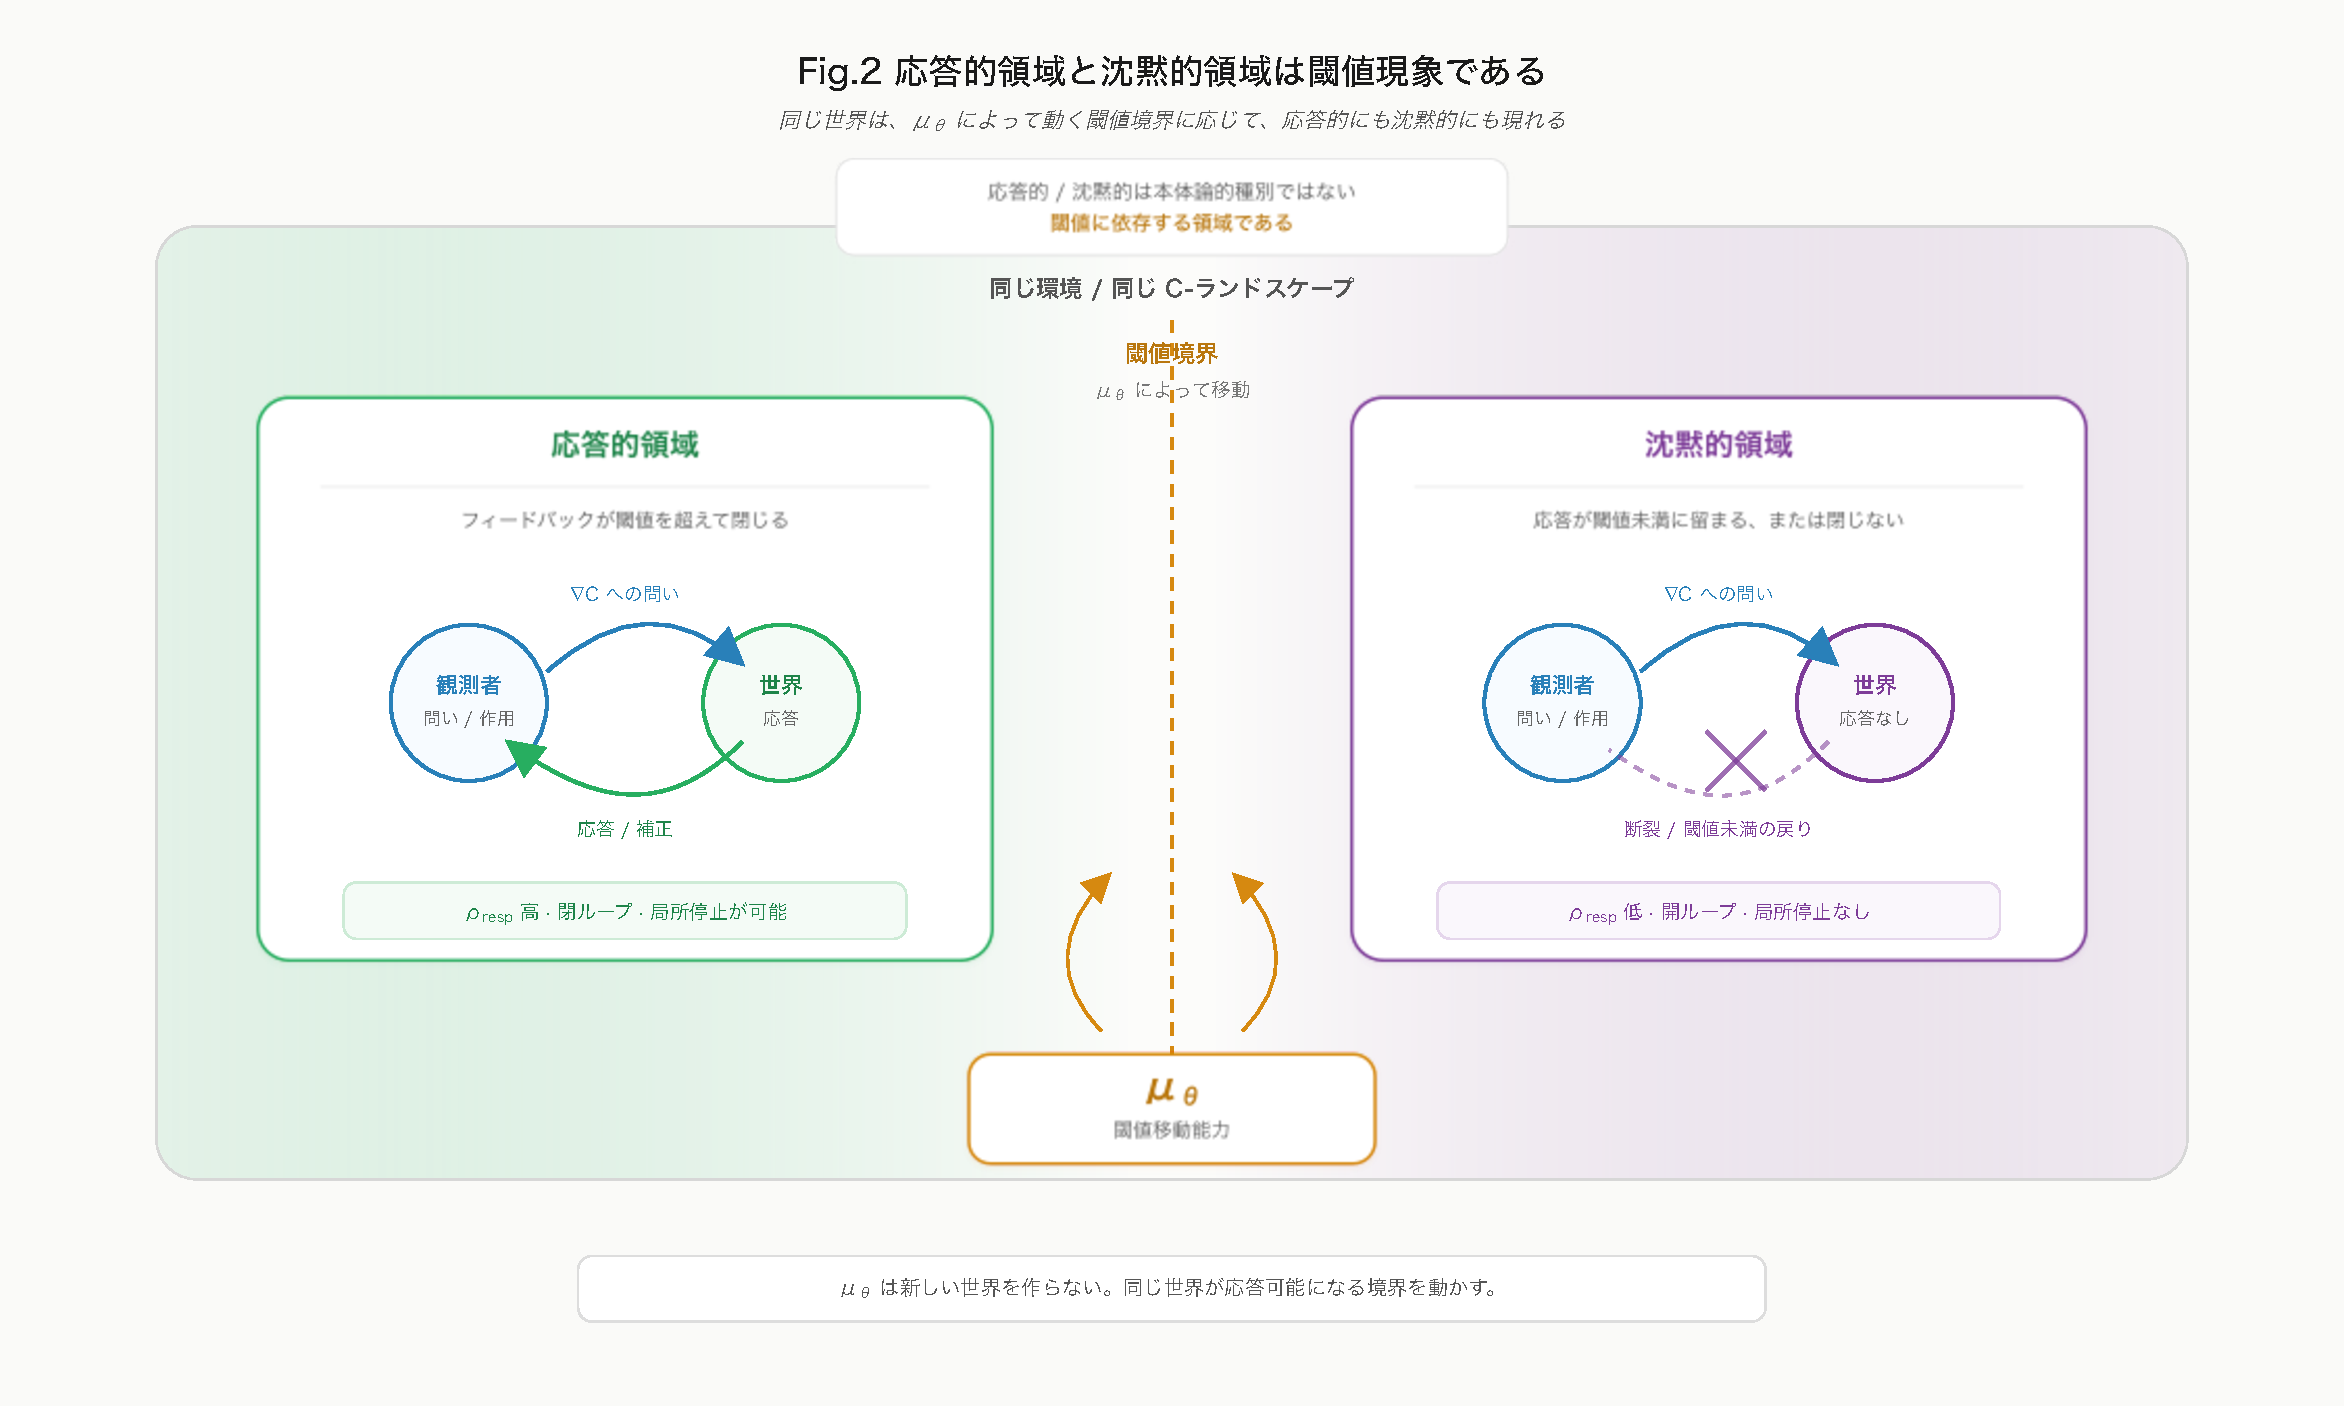
\includegraphics[width=\linewidth]{fig2_responsive_silent_threshold_ja.pdf}
\caption{応答的世界と沈黙的世界。両者は世界の存在論的な種別ではなく、$\mu_\theta$ が動かす閾値境界の左右にどちらが落ちるかで決まる相である。}
\label{fig:part2-responsive-silent}
\figurenote{左右は同一の環境とモデル内の $C$-地景を、異なる閾値境界で比較する模式図である。}{外部相互拘束と局所停止の関係は機能仮説であり、認知的停止や外化の必要性を図から導くものではない。}
\end{figure}

\bigskip


\subsection{沈黙世界における条件付きの無限後退解釈}


沈黙的世界に固定された推論主体——すなわち閾値を動かせず、環境を沈黙的として扱い続ける主体——を考える。この分類だけで以下が成立するとはせず、既述の旧局所状態模型の固定閾値・movement A・厳密増加の模型に沿って、次の条件付き解釈を検討する。

\textbf{条件 (1)}: 環境が応答を返さない(沈黙性、$H_{ji} \approx 0$)。

\textbf{条件 (2)}: 正当化は推論によってのみ生成される(\S{}3 の前提 P2)。

\textbf{条件 (3)}: 既述の固定閾値・movement A・厳密増加の模型で内部不動点不在を議論する。仮想的な停止述語 S の議論は、再評価演算子 F-prime にも前提を再適用できるかが未確立である(\S{}3 の定理 3.1、系 3.2)。

これらの条件と仮想的な停止模型を、無限後退という解釈の動機とする。任意の認知的停止の不可能性は結論しない。

解釈の依存関係は次の通りである。条件 (1) は外部応答の欠如、条件 (2) は正当化の供給源を限定する模型上の前提である。条件 (3) の不動点不在を停止一般の不在と同一視せず、仮想 S の再評価にも前提が引き継がれる場合の後退を考える。その再適用や認知的対応は未確立であり、無限後退を無条件の帰結とはしない。

これは \S{}3.5 の仮想停止模型を操作環境と比較する解釈である。\S{}3 の固定閾値・movement A・厳密増加および再評価への前提再適用という限定を保ち、\S{}4 では沈黙的世界に固定された主体への候補的解釈として提案する。現実発生の確認ではない。

\bigskip


\subsection{無限後退と分岐爆発の相同}


\S{}4.4 の無限後退は、Part I \S{}7 で導入された分岐爆発との役割上の類比である。

無限後退は非終端の軌道、分岐爆発は経路増大として別々に記述する。\S{}3.7 の比較は、内部不動点不在と両者を同一機構とする証明ではない:

\begin{itemize}
\item 固定閾値・movement A・厳密増加の模型での内部不動点不在を、無限後退という解釈と区別して比較する。仮想 S の再評価への前提再適用も未確立である
\item 確率構造(性質 F2)と経路の複数性の関係は候補的な対応であり、指数的分岐は別の条件を要する
\end{itemize}


回帰と分岐を組み合わせた認知的な不安定化は仮説である。沈黙的世界という分類や形式的不動点不在だけから、主体の経験する発散は導かれない。

過剰確信・麻痺・妄想的閉包との関係も候補的な解釈である。$L_E$ を欠いた $L_F$ の模型から、そのいずれかへの臨床的・認知的な必然的帰着は結論しない。

\bigskip


\subsection{ログ層 $L_R$ の予兆}


ここで、本論文の第二中心 \S{}5 の機構仮説を検討する動機が得られる。

旧局所状態模型の固定閾値・movement A・厳密増加という既述の模型の下での非閉包を、痕跡保持の可能性を検討する動機とする。推論軌道の記録——どの状態を経たか、どの分岐を試みたか、どこで発散したか——が保持される場合を考えるが、停止不在だけからその蓄積は導かれない。

以下の予兆から章末まで、保持痕跡は再帰利用の候補として読む。推論継続だけから保持・accessを得るのではない。activeなLR役割と一時的scaffoldの説明は第5節に置き、参照processそのものと区別する。保存する後退から層へのchainは旧仮説の動機であり、supportの同一性・参照可能性・LE形成を確立しない。

この堆積した痕跡を \textbf{ログ} と呼ぶ。そして、ログに対する再帰的な参照運動——過去の推論軌跡を読み返し、パターンを抽出し、現在の推論に反映する運動——が生じる層を、\textbf{ログ層} $L_R$ と呼ぶ(正式な定義は \S{}5.2)。

重要なのは、$L_R$ と $L_F$ の運動の関係を仮説化するという点である。$L_F$ の痕跡が保持されれば、再帰参照の候補となりうる。すなわち、$L_F$ の非閉包性と $L_R$ の形成は別であり、痕跡保持と再帰参照の機構を指定していない。保持された痕跡が再参照を支えうるという提案を、停止不在からの必然的な生成と区別する。

$L_F$ の停止未指定を、$L_F$ と別の層($L_R$)を検討する動機とする。\S{}5 では $L_R$ の再帰と外部相互拘束 $H_{ij}$ を創発停止層 $L_E$ の仮説に関連づける。$L_E$ が $L_F$ にない停止を実際に生成することは、この命名や形式的限界だけからは確認されない。

すなわち、無限後退は単なる行き詰まりではない。それは $L_R$ の形成と、$L_R$ を通じた $L_E$ の創発に関わるという仮説であり、生産性が導出された意味ではない。

\bigskip


\subsection{次章への橋渡し}


本章で仮説化する経路を以下に保存する。矢印は実行済み機構や存在・収束の証明ではない:

\[
L_F \text{の非閉包(§3)} \;\longrightarrow\; \text{沈黙世界での無限後退(§4.4)} \;\longrightarrow\; \text{ログの堆積} \;\longrightarrow\; L_R \text{の予兆(§4.6)}
\]

\S{}5 では $L_R$ と創発停止層 $L_E$ の関係を検討する。ログ層 $L_R$ の定義と、$L_E$ の機構仮説(閾値移動 $\mu_\theta$ の (B)、相互拘束 $H_{ij}$、停止演算子 $E$ の設置)を分ける。外部参照場 $\Phi_{\text{ext}}$ と個体間 $L_E$ ネットワーク $\Phi_{\text{net}}$ は二視点比較であり、同一性は未解決である。

\S{}3 の「$L_F$ の条件付き非閉包」と \S{}5 の「$L_E$ による停止の構成案」を分ける。\S{}4 は回帰と $L_R$ の関係を仮説化して両者を接続するが、動力学的生成や停止実現を示したものではない。

\bigskip


\subsection{要約}


本章で示したのは次の点である:

\begin{enumerate}
\item 推論環境は応答的世界($\nabla C$ 双方向閉ループ)と沈黙的世界($\nabla C$ 一方向)に区別される
\item 沈黙性は欠陥ではなく構造的なものである
\item しかし応答的/沈黙的は本体論的範疇ではなく、相互拘束パラメータ上の閾値現象である(\S{}2.6)
\item 沈黙・推論依存・停止未指定の三条件と問いの再適用を前提に、回帰を模型として検討する
\item 無限後退・分岐爆発・三つの病的引力子という認知的解釈は、異なる負担として分ける
\item 再帰運動とログ層 $L_R$ の関係を提案するが、形式的非閉包による高次層の生成証明ではない
\item $L_F$ の非閉包性と $L_R$ の形成、および \S{}5 の $L_E$ 創発は別の仮説である
\end{enumerate}


それでは \S{}5 において、本論文の第二中心——創発停止層 $L_E$ の動力学——を展開する。

\bigskip
